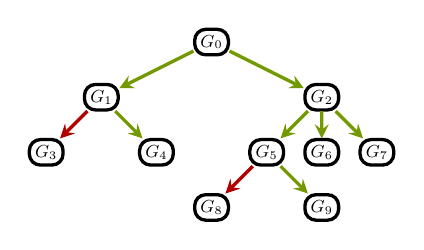
\begin{tikzpicture}[
    scale=0.7,
    transform shape,
    >=stealth,
    node distance=2.2cm and 2.5cm,
    hypernode/.style={draw, rectangle, rounded corners=4pt, very thick, inner sep=3pt, font=\small\bfseries},
    event/.style={draw=none, font=\normalsize},
    rf/.style={->, thick, dashed, green!60!black},
    co/.style={->, thick, dotted, red!80!black},
    graph box/.style={draw, rectangle, rounded corners=4pt, thick, minimum width=1.4cm, minimum height=1cm, inner sep=0.1cm, minimum size=0cm},
    edge label/.style={midway, very thick, fill=white, font=\footnotesize, inner sep=1pt},
    graph box yellow/.style={graph box, dashed},
    graph box blue/.style={graph box},
    every node/.style={transform shape},
    edge-t1/.style={->, very thick, lime!60!black},
    edge-t2/.style={->, very thick, red!70!black},
    circ-label-t1/.style={text=black, inner sep=1pt, font=\normalsize, scale=1.2},
    circ-label-t2/.style={text=black, inner sep=1pt, font=\normalsize, scale=1.2}
]


\node[hypernode] (G0) at (0,0) {$G_0$};

\node[hypernode] (G1) at (-2,-1) {$G_1$};

\node[hypernode] (G2) at (2,-1) {$G_2$};

\node[hypernode] (G3) at (-3,-2) {$G_3$};

\node[hypernode] (G4) at (-1,-2) {$G_4$};

\node[hypernode] (G5) at (1,-2) {$G_5$};

\node[hypernode] (G6) at (2,-2) {$G_6$};

\node[hypernode] (G7) at (3,-2) {$G_7$};

\node[hypernode] (G8) at (0,-3) {$G_8$};

\node[hypernode] (G9) at (2,-3) {$G_9$};



%% Hyper Edges

\draw[edge-t1] (G0) -- (G1);

\draw[edge-t1] (G0) -- (G2);

\draw[edge-t2] (G1) -- (G3);

\draw[edge-t1] (G1) -- (G4);

\draw[edge-t1] (G2) -- (G5);

\draw[edge-t1] (G2) -- (G6);

\draw[edge-t1] (G2) -- (G7);

\draw[edge-t2] (G5) -- (G8);

\draw[edge-t1] (G5) -- (G9);

\end{tikzpicture}
\captionof{figure}{The compressed transition system $\mathcal{D}(\ref{ex:lll})$}
\label{lll-comp}